% !TeX root = RJwrapper.tex
\title{Changes on CRAN}
\subtitle{%
2024-07-01 to 2024-09-30
}
\author{by Kurt Hornik, Uwe Ligges, and Achim Zeileis}
\maketitle
\section{CRAN growth}\label{cran-growth}
In the past 3 months, 473~new packages were
added to the CRAN package repository. 144~packages
were unarchived, 207~were archived and
1~had to be removed. The following shows the
growth of the number of active packages in the CRAN package repository:
\begin{center}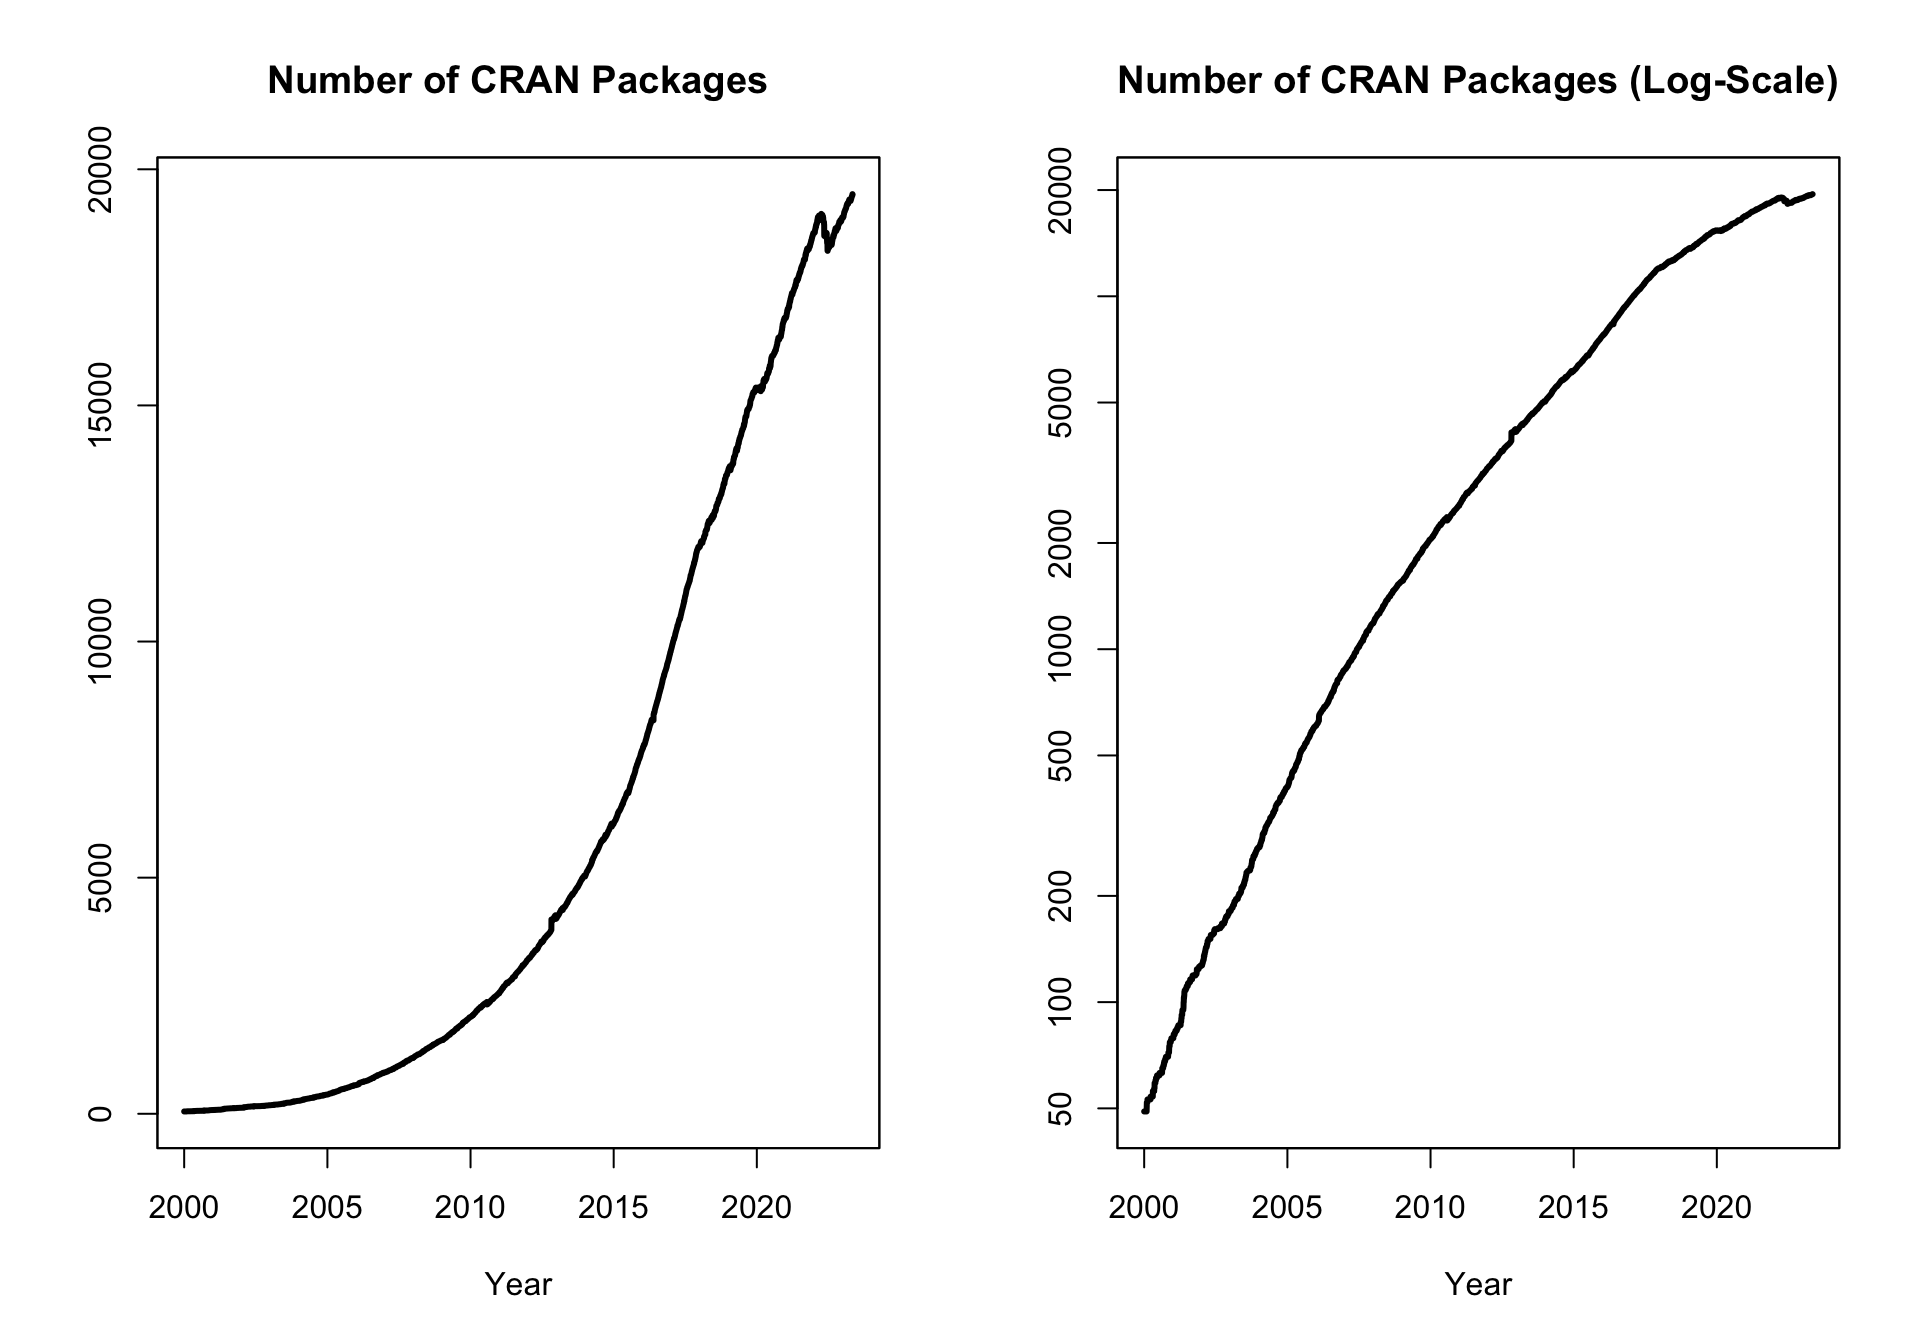
\includegraphics[width=1\linewidth,alt={CRAN growth: Number of CRAN packages over time in levels (left) and in logs (right).}]{RJ-2024-2-cran_files/figure-latex/cran_growth-1} \end{center}
\noindent On 2024-09-30, the number of active packages was around~21414.
\section{Changes in the CRAN Repository Policy}\label{changes-in-the-cran-repository-policy}
Similar to providing ORCID identifiers for individual authors and contributors in R packages,
the policy now encorages to provide ROR identifiers (from the Research Organization Registry,
\url{https://ror.org/}) in a package's \texttt{DESCRIPTION} file in case there are organizations among
the authors and contributors.
The policy now points out explicitly that package names on CRAN are persistent and in general
it is not permitted to change a package's name.
\section{CRAN package submissions}\label{cran-package-submissions}
From July 2024 to September 2024
CRAN received 6705~package submissions.
For these, 10875~actions took place of which
7759~(71\%) were auto processed actions and
3116~(29\%) manual actions.
Minus some special cases, a summary of the auto-processed and manually
triggered actions follows:
\begin{longtable}[]{@{}
  >{\raggedright\arraybackslash}p{(\columnwidth - 16\tabcolsep) * \real{0.0986}}
  >{\raggedleft\arraybackslash}p{(\columnwidth - 16\tabcolsep) * \real{0.1127}}
  >{\raggedleft\arraybackslash}p{(\columnwidth - 16\tabcolsep) * \real{0.1127}}
  >{\raggedleft\arraybackslash}p{(\columnwidth - 16\tabcolsep) * \real{0.1127}}
  >{\raggedleft\arraybackslash}p{(\columnwidth - 16\tabcolsep) * \real{0.1127}}
  >{\raggedleft\arraybackslash}p{(\columnwidth - 16\tabcolsep) * \real{0.1127}}
  >{\raggedleft\arraybackslash}p{(\columnwidth - 16\tabcolsep) * \real{0.1127}}
  >{\raggedleft\arraybackslash}p{(\columnwidth - 16\tabcolsep) * \real{0.1127}}
  >{\raggedleft\arraybackslash}p{(\columnwidth - 16\tabcolsep) * \real{0.1127}}@{}}
\toprule\noalign{}
\begin{minipage}[b]{\linewidth}\raggedright
\end{minipage} & \begin{minipage}[b]{\linewidth}\raggedleft
archive
\end{minipage} & \begin{minipage}[b]{\linewidth}\raggedleft
inspect
\end{minipage} & \begin{minipage}[b]{\linewidth}\raggedleft
newbies
\end{minipage} & \begin{minipage}[b]{\linewidth}\raggedleft
pending
\end{minipage} & \begin{minipage}[b]{\linewidth}\raggedleft
pretest
\end{minipage} & \begin{minipage}[b]{\linewidth}\raggedleft
publish
\end{minipage} & \begin{minipage}[b]{\linewidth}\raggedleft
recheck
\end{minipage} & \begin{minipage}[b]{\linewidth}\raggedleft
waiting
\end{minipage} \\
\midrule\noalign{}
\endhead
\bottomrule\noalign{}
\endlastfoot
auto & 2184 & 724 & 1459 & 219 & 0 & 2001 & 736 & 364 \\
manual & 1255 & 22 & 24 & 49 & 63 & 1282 & 351 & 58 \\
\end{longtable}
These include the final decisions for the submissions which were
\begin{longtable}[]{@{}lrr@{}}
\toprule\noalign{}
& archive & publish \\
\midrule\noalign{}
\endhead
\bottomrule\noalign{}
\endlastfoot
auto & 2046 (31.2\%) & 1717 (26.2\%) \\
manual & 1235 (18.8\%) & 1564 (23.8\%) \\
\end{longtable}
\noindent where we only count those as \emph{auto} processed whose publication or
rejection happened automatically in all steps.
\section{CRAN mirror security}\label{cran-mirror-security}
Currently, there are 94 official CRAN mirrors,
73~of which provide both
secure downloads via `\texttt{https}' \emph{and} use secure mirroring from the CRAN master
(via rsync through ssh tunnels). Since the~R 3.4.0 release, \texttt{chooseCRANmirror()}
offers these mirrors in preference to the others which are not fully secured (yet).
\section{CRAN Task View Initiative}\label{cran-task-view-initiative}
There is one new task view:
\begin{itemize}
\tightlist
\item
  \href{https://CRAN.R-project.org/view=DynamicVisualizations}{Dynamic Visualizations and Interactive Graphics}: Maintained by Sherry Zhang, Dianne Cook, Ian Lyttle.
\end{itemize}
Currently there are 46~task views (see \url{https://CRAN.R-project.org/web/views/}),
with median and mean numbers of CRAN packages covered
110 and~123, respectively.
Overall, these task views cover 4741~CRAN packages,
which is about 21\% of all active CRAN packages.
\address{%
Kurt Hornik\\
WU Wirtschaftsuniversität Wien\\%
Austria\\
%
%
\textit{ORCiD: \href{https://orcid.org/0000-0003-4198-9911}{0000-0003-4198-9911}}\\%
\href{mailto:Kurt.Hornik@R-project.org}{\nolinkurl{Kurt.Hornik@R-project.org}}%
}
\address{%
Uwe Ligges\\
TU Dortmund\\%
Germany\\
%
%
\textit{ORCiD: \href{https://orcid.org/0000-0001-5875-6167}{0000-0001-5875-6167}}\\%
\href{mailto:Uwe.Ligges@R-project.org}{\nolinkurl{Uwe.Ligges@R-project.org}}%
}
\address{%
Achim Zeileis\\
Universität Innsbruck\\%
Austria\\
%
%
\textit{ORCiD: \href{https://orcid.org/0000-0003-0918-3766}{0000-0003-0918-3766}}\\%
\href{mailto:Achim.Zeileis@R-project.org}{\nolinkurl{Achim.Zeileis@R-project.org}}%
}
